%%%%%%%%%%%%%%%%%%%%%%%%%%%%%%%%%%%%%%%%%
%%%%%%%%%% Content starts here %%%%%%%%%%
%%%%%%%%%%%%%%%%%%%%%%%%%%%%%%%%%%%%%%%%%

\begin{frame}{Преглед}
	\begin{itemize}[<+-| alert@+>]
	  \item Мотивација
	  \item Што е Е-Лаб?
	  \item Технички проблеми и решенија
	  \item Филозофија на дизајнот на Е-Лаб
	  \item Архитектура
	  \item Е-Лаб 2.0
	  \item Заклучок
	\end{itemize}
\end{frame}

\begin{frame}{Мотивација}
	\begin{itemize}[<+-| alert@+>]
	  \item Програмирањето е една од основните практични вештини која што се
	  изучува во програмите на информатичките факултети и секундарна вештина на
	  многу други технички факултети
	  \item Големата побарувачка на пазарот на трудот за програмери е една од
	  причините за интересот и популарноста меѓу идните студенти
	  \item Резултат се големи групи студенти во воведните курсеви
	  \item А програмирањето не е лесно!
	  \item Потребно е да се решат голем број основни алгоритамски проблеми
	  (повеќе од една третина од времето)
	\end{itemize}
\end{frame}

\begin{frame}{Идентификација на проблемот}
	\begin{itemize}[<+-| alert@+>]
	  \item Контекстот
	  \begin{itemize}
	  	\item 500+ студенти
	  	\item Поделба во групи од  20
	  	\item Решавање на 3 - 6 задачи неделно
		\end{itemize}
		\item Проблемите
	  \begin{itemize}
	  \item Секој инструктор треба да прегледа и оцени до 120 решенија за 15-30
	  минути
	  \item Недостиг на повратна информација кон студентите
	  \item Дефокусурање на студентите од решавање на проблемите и недостиг на
	  мотивација
	 \end{itemize}
	\end{itemize}
\end{frame}

\begin{frame}{Што е Е-Лаб?}
    \begin{itemize}[<+-| alert@+>]
      \item \emph{Е-Лаб} е веб базиран систем за решевање и автоматско прегледување
      и оценување задачи од воведни курсеви за програмирање (можност за
      изведување испити)
      \item Сѐ што е потребно е веб прелистувач
      \item Централизирана автентикација со можност за отворен или ограничен
      пристап (CAS)
      \item Систем за контрола на верзиите на задачите и решенијата
      \item Безбедно извршување (Sandbox)
      \item Подршка за различни видови задачи во повеќе програмски јазици (C, C++,
      Java)
      \item Развиен за скалабилност и проширување
    \end{itemize}
\end{frame}

% Define block styles
\tikzstyle{block} = [rectangle, draw, fill=blue!20,
text width=5em, text centered, rounded corners, minimum height=4em]
\tikzstyle{line} = [draw, -latex']

\begin{frame}[fragile]{Решение}
	\begin{itemize}
  	  \item Алгоритамски видови на задачи
	\end{itemize}
\begin{center}
\begin{tikzpicture}[node distance = 3cm, auto]
    % Place nodes
    \pause
    \node [block] (input) {Влез};
    \pause     
    \path [line] (input) -> node {} (algorithm);
    \node [block, right of=input] (algorithm) {Алгоритам}
    \pause
    \path [line] (algorithm) -> node {} (output);
    \node [block, right of=algorithm] (output) {Излез};
    % Draw edges
\end{tikzpicture}
\end{center}
\pause
\begin{itemize}[<+->]
  \item Се користи во системи за натпревари во програмирање
  \item Ја потенцираат важноста во програмирањето да се има решение
  кое работи точно
\end{itemize}
\end{frame}


\begin{frame}{Целите на Е-Лаб}
	\begin{itemize}[<+-| alert@+>]
	  \item Подобра организација и имплементација на вежбите и испитите кои
	  вклучуваат програмирање
	  \item Мотивирање на студентите со постојана повратна информација за
	  точноста на нивните решенија
	  \item Поместување на улогата на инструкторите од едноставни учители и
	  оценувачи до поголеми мотиватори
	\end{itemize}
\end{frame}

\begin{frame}{Интегриран поглед на задачата}
	\begin{figure}
		\centering
		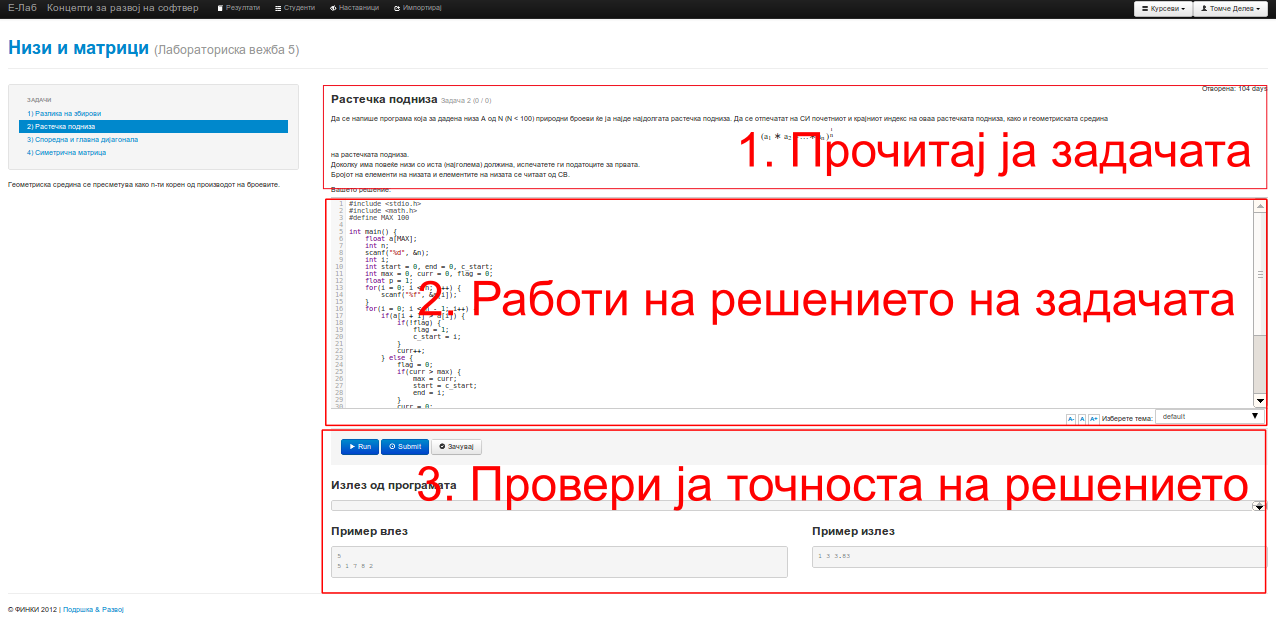
\includegraphics[width=.99\textwidth]{images/pv}
		\caption{Погледот на студентот кој се обидува да реши задача}
		\label{fig:student_screen}
	\end{figure}
\end{frame}

\begin{frame}{Архитектура на системот}
	\begin{figure}
	\centering
		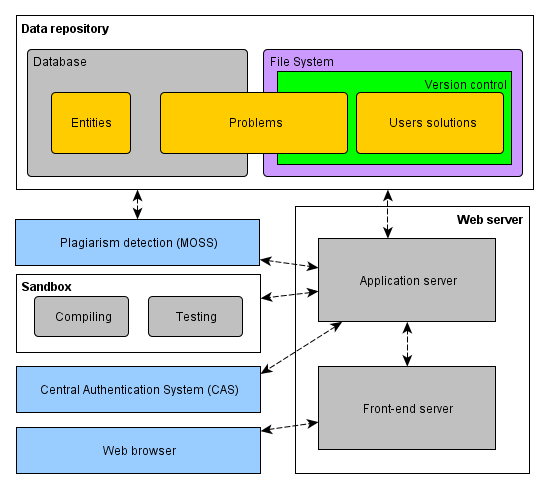
\includegraphics[width=.70\textwidth]{images/architecture}
		\caption{Архитектура на Е-Лаб.}
		\label{fig:architecture}
	\end{figure}
\end{frame}

\begin{frame}{Податоци за користење на Е-Лаб}
\begin{itemize}
  \item 1391 корисници
    \begin{itemize}
    \item 1344 студенти
    \item 33 демонстратори
    \item 12 наставници и асистенти
    \item 2 администратори
    \end{itemize}
    \item > 220 задачи
    \item > 30000 уникатни погледи на задачи
    \item > 86000 обиди за решавање
    \begin{itemize}
        \item > 29000 точни
    \end{itemize}
\end{itemize}
\end{frame}

\begin{frame}{Погледи во последниот месец}
    \begin{figure}
    \centering
        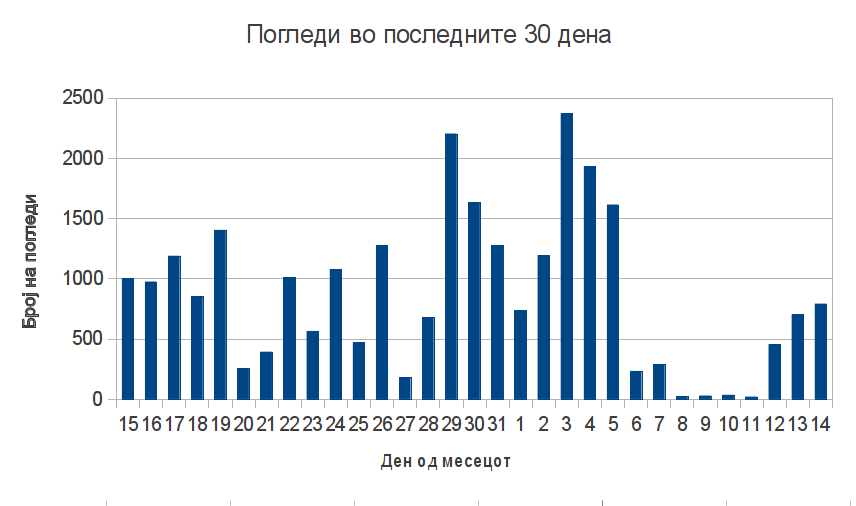
\includegraphics[width=.99\textwidth]{images/views}
    \end{figure}
\end{frame}

\begin{frame}{Обиди во последниот месец}
    \begin{figure}
    \centering
        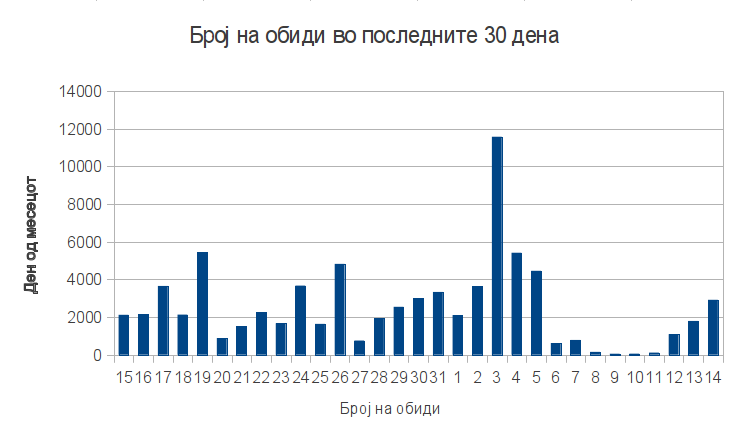
\includegraphics[width=.99\textwidth]{images/attempts}
    \end{figure}
\end{frame}

\begin{frame}{Понатамошна работа 1/2}{Насоки за истражување}
\begin{itemize}[<+-| alert@+>]
  \item Надградба во систем за учење Е-Лаб 2.0
  \item Поголема интерактивност во процесот на тестирање
  \item Машинско учење во системот и автоматско препознавање на најчестите
  грешки
  \item Автоматска детекција на плагијати
  \item Дополнителна биометриска автентикација преку начинот на користење на
  тастатурата
\end{itemize}
\end{frame}

\begin{frame}{Понатамошна работа 2/2}{Насоки за истражување}
\begin{itemize}[<+-| alert@+>]
  \item Поврзување на студентите, инструкторите и наставниците
  \item Создавање на мрежа за колаборација 
  \begin{itemize}
  \item едноставна комуникација
  \item меѓусебно оценување (peer review)
  \item прегледување на решенијата (code review)
  \end{itemize}
  \item Истражување на можностите за интерактивна комуникција
  \begin{itemize}
  \item споделување кратки пораки (chat)
  \item споделување на состојбата преку листа од акции кои се извршени
  \end{itemize}
  \item Анализа и обработка на податоците од комуникацијата меѓу студентите во
  корелација со нивните резултати и оценки
\end{itemize}
\end{frame}

\begin{frame}{Заклучок}
	\begin{itemize}[<+-| alert@+>]
	  \item Директно решавање на големи организациони проблеми
	   \begin{itemize}
	   \item просторни проблеми
	   \item инфраструктурни и технички проблеми
	  \end{itemize}
	  \item Поедноставување на процесот на создавање и управување со
	  многу оригинални задачи од програмирање
	  \item Централизиран репозиториум со задачи и решенија од сите студенти
	  (истовремено со можност за дистрибуираност)
	  \item Постојана достапност и можност за скалирање
	  \item Создавање огромно количество на податоци за начинот на учење,
	  интеракцијата, нивото на комуникација помеѓу студентите, инструкторите и
	  наставниците
	\end{itemize}
\end{frame}

\begin{frame}{Прашања}{}
	\begin{center}
	\Large{
    \href{http://e-lab.finki.ukim.mk/}{\textbf{http://e-lab.finki.ukim.mk}}}
    \vfill
    \huge{Ви благодарам}
    \vfill    
    \Huge{Прашања?}
	
	\end{center}
\end{frame}

